\chapter{Automatización de tareas}

\section{Automatización en scripts bash}
\subsection{Automatizar la clonación del proyecto}

Para automatizar la obtención del código fuente del proyecto se implementó
el script \texttt{clone-project.sh}, ubicado en la raíz del repositorio.
Este script permite clonar automáticamente el repositorio de MoonPhases
sin necesidad de ejecutar manualmente el comando de clonación.

El contenido del script es el siguiente:

\begin{lstlisting}[language=bash]
#!/bin/bash

REPO_URL="https://github.com/Angello599/MoonPhases-DevOps.git"
PROJECT_DIR="MoonPhases-DevOps"

echo "======================================"
echo "   CLONANDO PROYECTO MOONPHASES"
echo "======================================"

if [ -d "$PROJECT_DIR" ]; then
    echo "El directorio $PROJECT_DIR ya existe."
    exit 1
fi

git clone "$REPO_URL" "$PROJECT_DIR"

if [ $? -eq 0 ]; then
    echo ""
    echo "======================================"
    echo "   PROYECTO CLONADO CORRECTAMENTE"
    echo "======================================"
else
    echo ""
    echo "======================================"
    echo "   ERROR AL CLONAR EL PROYECTO"
    echo "======================================"
    exit 1
fi
\end{lstlisting}

El script define la URL del repositorio y el nombre del directorio donde se
almacenará el proyecto. Antes de realizar la clonación, verifica si el
directorio de destino ya existe para evitar sobrescribir una copia
existente. Si el directorio no existe, ejecuta \texttt{git clone} para
descargar el repositorio. Finalmente, verifica el código de salida de la
operación e informa si la clonación se realizó correctamente o si ocurrió
un error.

Para ejecutar el script se utiliza el siguiente comando desde Git Bash:

\begin{lstlisting}[language=bash]
./clone-project.sh
\end{lstlisting}

De esta manera, la clonación del repositorio queda automatizada mediante un
script Bash y puede ejecutarse utilizando un único comando.

\begin{figure}[H]
    \centering
    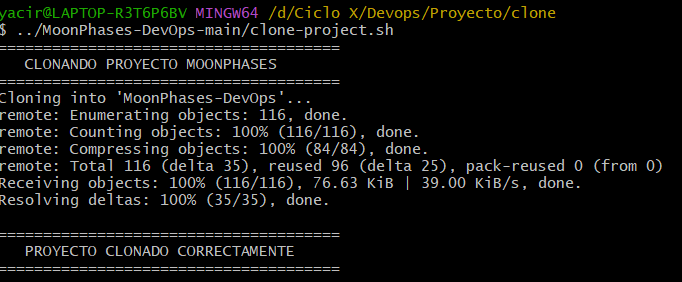
\includegraphics[width=0.80\textwidth]{content/imgs/k3.png}
    \caption{Automatización de clonación del proyecto.}
\end{figure}

\subsection{Automatizar la ejecución de los test}

Para automatizar la ejecución de las pruebas unitarias se implementó el
script \texttt{run-tests.sh}, ubicado en la raíz del repositorio. Este
script permite ejecutar las pruebas mediante un único comando y verificar
automáticamente si fueron ejecutadas correctamente.

El contenido del script es el siguiente:

\begin{lstlisting}[language=bash]
#!/bin/bash

echo "======================================"
echo "   EJECUTANDO TESTS DE MOONPHASES"
echo "======================================"

npm test

if [ $? -eq 0 ]; then
    echo ""
    echo "======================================"
    echo "   TODOS LOS TESTS PASARON"
    echo "======================================"
else
    echo ""
    echo "======================================"
    echo "   ALGUN TEST FALLO"
    echo "======================================"
    exit 1
fi
\end{lstlisting}

El script ejecuta el comando \texttt{npm test}, que inicia Vitest y ejecuta
las nueve pruebas unitarias implementadas. Posteriormente, se verifica el
código de salida del proceso. Si el resultado es exitoso, se muestra un
mensaje indicando que todas las pruebas pasaron. En caso contrario, el
script informa que alguna prueba falló y finaliza con código de error.

Para ejecutar la automatización se utiliza:

\begin{lstlisting}[language=bash]
./run-tests.sh
\end{lstlisting}

El archivo se encuentra directamente en la raíz del proyecto, permitiendo
que la ejecución de las pruebas sea reproducible sin necesidad de ejecutar
cada prueba individualmente.

\begin{figure}[H]
    \centering
    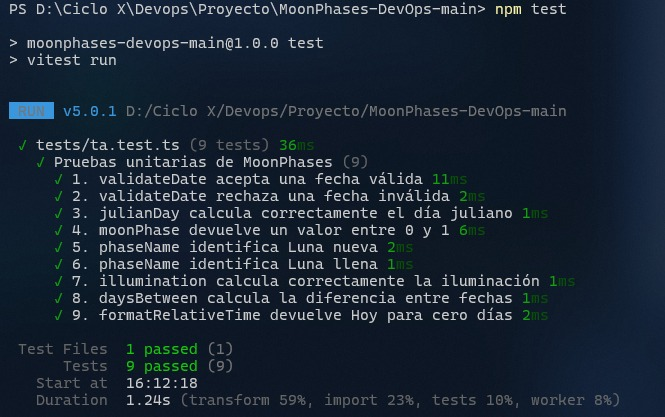
\includegraphics[width=0.80\textwidth]{content/imgs/k1.jpeg}
    \caption{Automatización de ejecución de test.}
\end{figure}


\subsection{Automatizar correr el proyecto en modo local}

Para automatizar el levantamiento del proyecto en modo local se implementó
el script \texttt{run-local.sh}, ubicado en la raíz del repositorio. Este
script permite iniciar los servicios de MoonPhases mediante Docker Compose
sin necesidad de ejecutar manualmente los comandos correspondientes.

El contenido del script es el siguiente:

\begin{lstlisting}[language=bash]
#!/bin/bash

echo "======================================"
echo "   LEVANTANDO MOONPHASES EN LOCAL"
echo "======================================"

if ! command -v docker &> /dev/null
then
    echo "ERROR: Docker no está instalado o no está disponible."
    exit 1
fi

docker compose up --build -d

if [ $? -eq 0 ]; then
    echo ""
    echo "======================================"
    echo "   MOONPHASES SE EJECUTA EN LOCAL"
    echo "======================================"
    echo ""
    echo "Frontend:"
    echo "http://localhost:8080/MoonPhases/"
    echo ""
    echo "Backend:"
    echo "http://localhost:3001/api/health"
else
    echo ""
    echo "======================================"
    echo "   ERROR AL LEVANTAR EL PROYECTO"
    echo "======================================"
    exit 1
fi
\end{lstlisting}

El script verifica inicialmente que Docker se encuentre disponible. Luego
ejecuta el comando \texttt{docker compose up --build -d}, mediante el cual
se construyen las imágenes necesarias y se levantan los servicios definidos
en el archivo \texttt{compose.yaml} en segundo plano.

Para ejecutar el script se utiliza el siguiente comando desde la raíz del
proyecto:

\begin{lstlisting}[language=bash]
./run-local.sh
\end{lstlisting}

\begin{figure}[H]
    \centering
    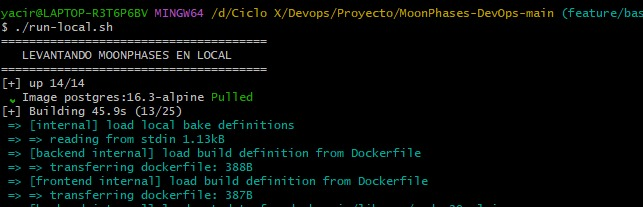
\includegraphics[width=0.9\textwidth]{content/imgs/run-loca.jpg}
        \caption{Automatización para correr el proyecto local.}
\end{figure}